\chapter{A Unified Graphical Model}

\label{ch:crf}


In this chapter, we propose to use a unified graphical model to model the interactions among regions. We start from a discussion on the major flaw of previous flow augmented spatial autoregressive model, that as a global spatial model is assumes spatial stationarity. However, in the real problem there is usually a spatial non-stationarity over some properties. For example, we observe that the relationship between crime count and total population in each community presents such spatial non-stationarity.

To fix the spatial non-stationarity issue, the most widely used method is called \emph{geographically weighted regression} (GWR) in the literature. In the next section, we will discuss the pros and cons to employ GWR to capture the spatial non-stationarity. Since our problem has multiple ``hyperlink'' flows in addition to space continuity, the idea of GWR must be generalized over a high dimension space consisted of multiple interactions. However, this generalization is non-trivial, and thus we propose a graphical model to address this challenge.



The graphical model is a natural way to capture the complicated interactions among regions.
With the same graphical model, we further show that other data mining tasks in urban space can be solved as well.  Therefore, we believe this graphical model is superior than other model in capturing the interactions, which consequently could be a united model.



\section{Capture Spatial Non-stationarity}

\subsection{Global Model vs. Local Model}

\begin{figure}[h]
\centering
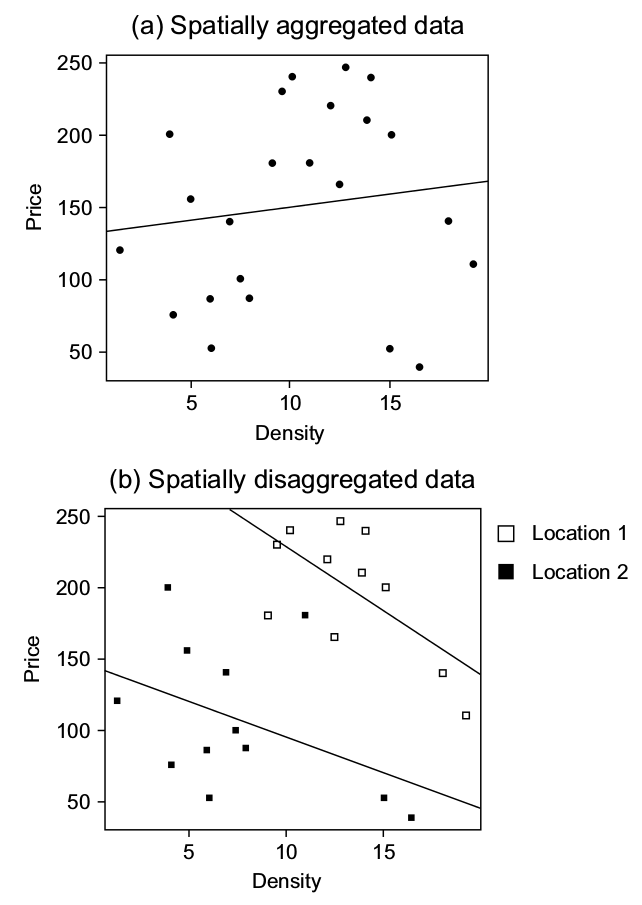
\includegraphics[width=0.7\textwidth]{fig/simpson.png}
\caption{A spatial example of Simpson's Paradox (from~\cite{GWR03}).}
\label{fig:simpson}
\end{figure}

\begin{figure}[h]
\centering
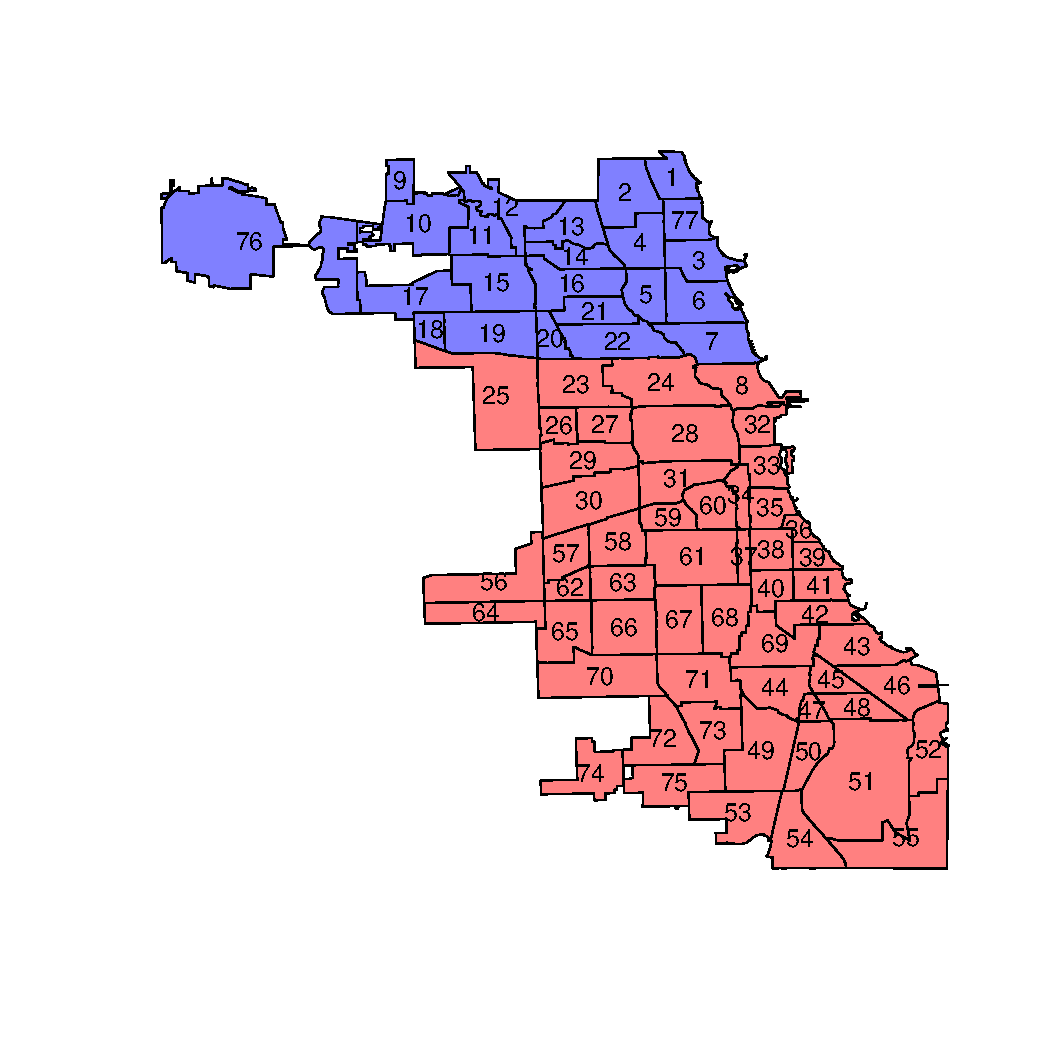
\includegraphics[width=0.45\textwidth]{fig/north-south-split.pdf}
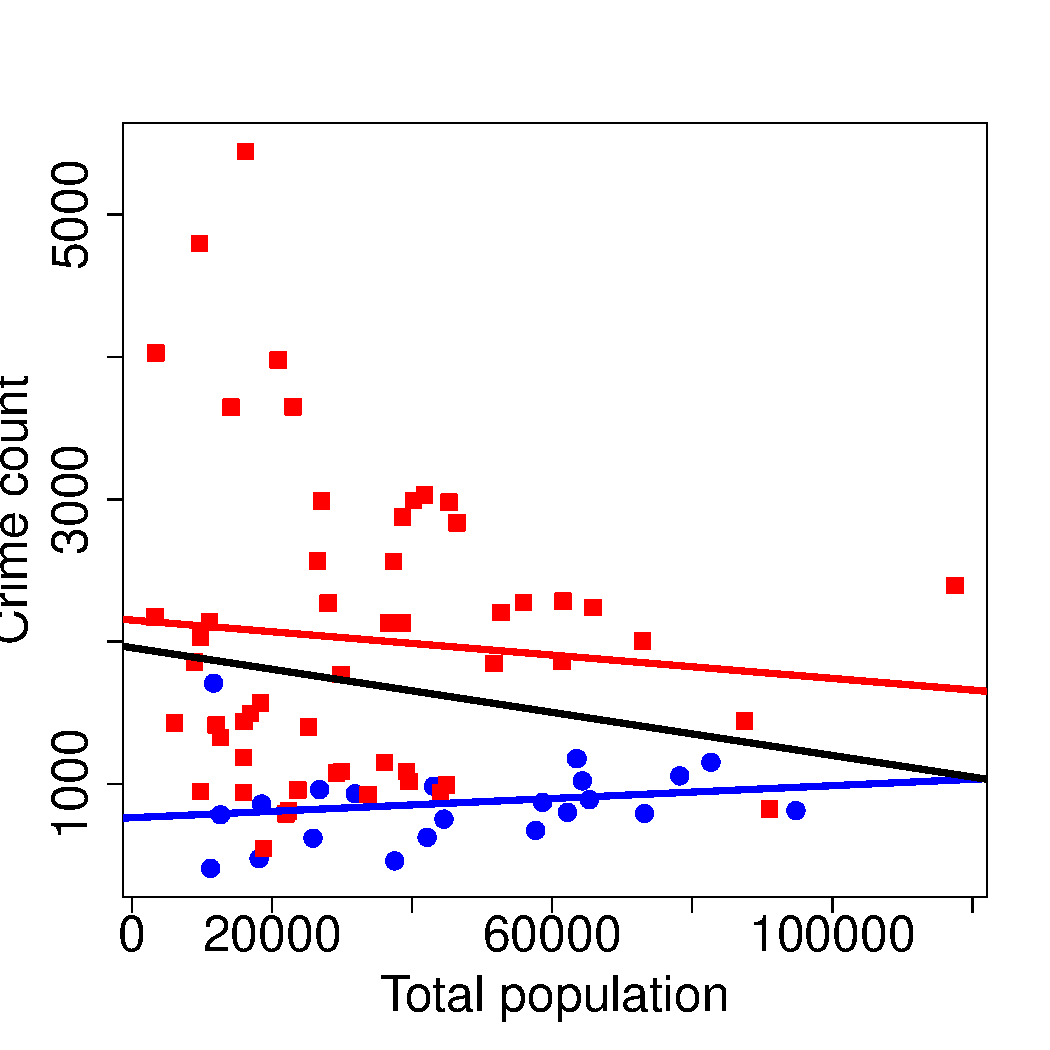
\includegraphics[width=0.45\textwidth]{fig/crime-pop.pdf}
\caption{The crime count vs. total population relationship shows spatial non-stationary property.}
\label{fig:spa-non-sta}
\end{figure}


Global model assumes the statistical relationships does not change over space. However, some statistical relationship is not stationary over space, which requries specific treatment for different locations, i.e. a local model at different places.



According to \cite{GWR03}, using global estimates of statistics can present misleading interpretations of local models. This is shown as an example in Figure~\ref{fig:simpson}, known as Simpson's Paradox~\cite{wiki:simpson}. The reason of Simpson's Paradox is that there is a hidden distribution of properties over space, which leads to opposite results in global model when aggregate subgroups over space.





In the Chicago crime inference example, we also observed similar phonomenon, as shown in Figure~\ref{fig:spa-non-sta}. We divide Chicago into two half: i) downtown north, ii) downtown and downtown south. The intuition is that the Chicago south usually have more crime than north, therefore we want to split Chicago into low-crime half and high-crime half. The splition of Chicago communites are visualized in left figure of Figure~\ref{fig:spa-non-sta}. 
On the right of Figure~\ref{fig:spa-non-sta}, we present the total crime plotted against total population. It is clear that in the high-crime half of Chicago the relation is almost neutral (coefficient as 0), and in the low-crime half of Chicago the relation is postive. However, the global model (black line) presents a negative correlation.





\subsection{An Existing Solution: Geographically Weighted Regression}


Geographically weighted regression (GWR) is a term introduced in \cite{GWR03} to describe a family of regression method in which the coefficients $\beta$ are allowed to vary spatially. GWR uses the coordinates of each sample or zone centroid $t_i$, as a target point for a form of spatially weighted least squares regression. The model is of the form:

\begin{equation}
y = X \beta(t) + \epsilon
\end{equation}

The coefficient $\beta(t)$ are determined at different regression point locally by its neighboring sample points. A weighting schema or spatial kernel $W$ is employed to weight neighboring sample points accordint to its distance to regression point. The Figure~\ref{fig:spa-kernel} is an example of the weighting function.


\begin{figure}[h]
\centering
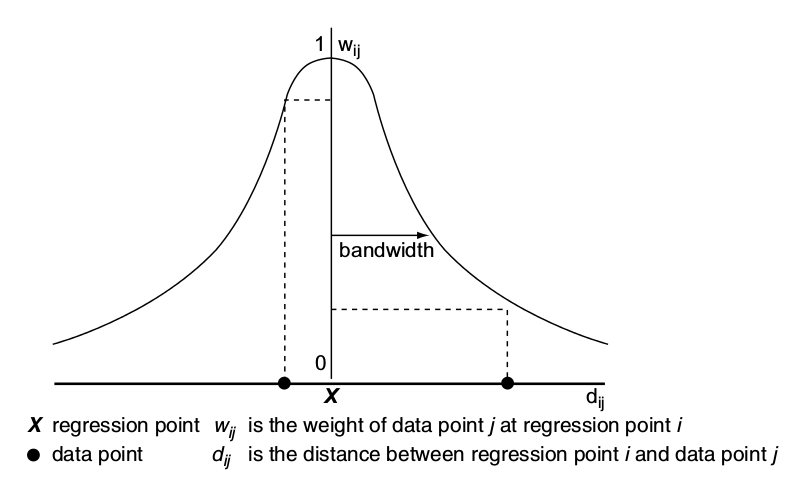
\includegraphics[width=0.8\textwidth]{fig/spatial-kernel.png}
\caption{A spatial kernel. Example from ~\cite{GWR03}}
\label{fig:spa-kernel}
\end{figure}



The GWR idea is able to be applied on top of spatial autoregressive (SAR) model, so that SAR model deals with spatial non-stationarity.  In the next we discuss another similar model called adaptive spatial model. After that, we discuss a common drawbacks of this two models.


\subsection{An Alternative Solution: Adaptive Spatial Model}


We use various types of data to estimate the crime count in community area (CA) of Chicago. For each CA we have observations on crime count and demographics. For each pair of CAs we also have observations on the taxi flow and spatial distance. One straightforward method is to build a regression model from all the features we observed to the crime counts.

We have one interesting observations is that in the south and north part of Chicago, the significance of different features are different. Therefore, the idea is to learn a dynamic weights for different spatial region.



Suppose we have $n$ regions in total, $R = \{ r_1, r_2, \cdots, r_n \}$.
The following notations are used

\begin{table}[h]
\centering
\begin{tabular}{|l|r|}
\hline
crime count at $r_i$ & $y_i$ \\ \hline
demographics at $r_i$ & $\mathbf{d}_i$ \\ \hline
taxi flow between $r_i$ and $r_j$ & $f_{ij}$ \\ \hline
taxi flow weight matrix for $r_i$ & $\mathbf{f_i}$ \\ \hline
spatial weight matrix for $r_i$ & $\mathbf{g_i}$ \\ \hline
social flow lag variable for $r_i$ & $s_i = \mathbf{f}_i^T \mathbf{y}$ \\\hline
spatial flow lag variable for $r_i$ & $p_i = \mathbf{g}_i^T \mathbf{y}$ \\\hline
\end{tabular}
\caption{Symbols for the dynamic coefficient model.}
\end{table}


\textbf{Dynamic linear regression model}



For simplicity we use linear regression model
\[
y_i = \mathbf{w}_1^T \mathbf{d}_i + w_2 s_i + w_3 p_i + w_4,
\]
where $\{ w \}$ are the coefficients.

To simplify notations, we use $\mathbf{x}_i$ denote all the available predictors for region $r_i$,
\[
\mathbf{x}_i = [ \mathbf{d}_i, s_i, p_i, 1 ].
\]
Then the model becomes 
\[
y_i = \mathbf{w}^T \mathbf{x}_i.
\]



Now we use a dynamic model, where $\mathbf{w}$ is different for various regions.
This leads to 
\[
y_i  = \mathbf{w}_i^T \mathbf{x}_i.
\]


The problem with formulation is that there are too many parameters to learn. To address this issue, we use the constraint that \textbf{spatially adjacent regions share similar coefficients}.

We use $S_{ij}$ to denote the adjacency of $r_i$ and $r_j$. And the aforementioned constraint is formulated as
\[
\min \sum_{i,j} S_{ij} ||\mathbf{w}_i^T - \mathbf{w}_j^T||_2^2
\] The several choice of $S_{ij}$
\begin{itemize}
\item Binary indicator. $S_{ij} = 1$ if two regions are contiguous, otherwise $S_{ij} = 0$.
\item The reverse distance between $r_i$ and $r_j$. 
\end{itemize}

The overall objective is

\begin{equation}
\label{eq:obj}
\min_{\mathbf{W}}  \sum_i || y_i - \mathbf{w}_i^T \mathbf{x}_i ||_2^2 + \eta \sum_{i,j} S_{ij} ||\mathbf{w}_i^T - \mathbf{w}_j^T||_2^2 
+ \theta || \mathbf{W} ||_F^2
\end{equation}




\textbf{Optimization}


Rewrite the Frobenius norm in the last term
\[
|| \mathbf{W} ||_F^2 = \sum_i || \mathbf{w}_i - \mathbf{0}||_2^2.
\]


Therefore the Equation~\ref{eq:obj} is rewritten as
\begin{equation}
\label{eq:obj2}
\min_{\mathbf{W}}  \sum_i || y_i - \mathbf{w}_i^T \mathbf{x}_i ||_2^2 + \eta \sum_{i,j \in 0, \cdots, N} S_{ij} || \mathbf{w}_i - \mathbf{w}_j ||_2^2,
\end{equation}
where $\mathbf{w}_0 = \mathbf{0}$ and $S_{0i} = 1$ for $\forall i$.


To solve the objective in Equation~\ref{eq:obj2}, we use variable splitting. Namely, when optimizing for $\mathbf{w}_i$, we assume all other $\mathbf{w}_{j, j\neq i}$ are fixed. The sub-problem is
\begin{equation}
\label{eq:subobj}
\min_{\mathbf{w}_i}   ||y_i - \mathbf{w}_i^T \mathbf{x}_i ||_2^2 + \eta \sum_j S_{ij}|| \mathbf{w}_i - \mathbf{w}_j||_2^2.
\end{equation}



The update on $\mathbf{w}_i$ is
\[
\mathbf{w}_i = \min_{\mathbf{w}_i}   ||y_i - \mathbf{w}_i^T \mathbf{x}_i ||_2^2 + \eta \sum_j S_{ij} || \mathbf{w}_i - \mathbf{w}_j^{(t)} ||_2^2.
\]

The closed-form solution is

\begin{equation}
\mathbf{w}_i = (\mathbf{x}_i^T \mathbf{x}_i + \eta \sum_j S_{ij} \mathbf{I} )^{-1} (y_i \mathbf{x}_i + \eta \sum_j S_{ij} \mathbf{w}_j) 
\end{equation}


\textbf{Inference}

We use the \textbf{leave-one-out} setting to infer and evaluate the crime rate of new community area. 

Suppose the we want to estimate the crime rate $y_i$ of $CA_i$. During the training process, we hold everything about $CA_i$ out (including $y_i$, flow coming in and leaving from $CA_i$). Then training the model on $CA_j$, $\forall j \neq i$, which gives us $w_j$, $\forall j \neq i$. To infer the $y_i$, we need estimate the model coefficient $w_i$ first. Follow the same intuition that model on $CA_i$ is only similar to all its neighboring models, we have
\begin{equation}
\min_{\mathbf{w}_i} \sum_{j, \forall j \neq i} S_{ij} || \mathbf{w}_i - \mathbf{w}_j ||_2^2 + || \mathbf{w}_i ||_2^2
\end{equation}

After getting $\mathbf{w}_i$, we infer $y_i$ by
\begin{equation}
\hat{y}_i = \mathbf{w}_i^T * \mathbf{x}_i
\end{equation}




\subsection{Comparison of GWR and Adaptive Model}


Both the GWR and Adaptive model address the spatial non-stationarity by building local models. Two models use different approaches to model the spatial continuity.

GWR implicitly model the spatial continuity by using similar sample points for two nearby regression models. Meanwhile, the adaptive model explicitly put a constrait to make two nearby models similar.

Both mehtods can be extened with newer type of interactions. We use $W^0$ denote the spatial adjacency matrix, and use $W^k$, $k = 1,2, \cdots$ to denote the interactions matrix of data type $k$. Therefore, we are extending the two dimensional distance weighting kernel into a high dimension distance measure. 


However, this high dimension distance measure is non-trivial to calculate. Suppose now we have taxi flow and LEHD flow in addition to geospatial adjacency. The tricky question to ask is which interaction is more important to connect two regions? We can give weight coefficient to different interactions, so that

\begin{equation}
W =  \alpha_0 W^0 + \alpha_1 W^1 + \cdots  +\alpha_k W^k
\end{equation}
where $\sum_0^k \alpha_i = 1$.

However, the $W$ in both GWR and adaptive model is pre-given. Therefore, incorporating heterogeneous flows is the major challenge of both GWR and adaptive model.




\section{Graphical Model to Capture Complicated Interactions}



The methods in the literature is not originally designed to handle heterogenous interactions among regions, and therefore have the major challenge mentioned above. The heterogenous interactions generate different network structure for us.  Therefore, we propose to model the interactions of two regions as a latent variables with a graphical model. 




\subsection{Problem Formulation}

We want to predict the crime rate $y_i$ of each geographical grid (tract/community area) $g_i$. The available observations are demographics features $\x_i$ of each $g_i$ from census, and the interactions among grids. We denote the interactions as $\f_{ij}$ for grid pair $g_i, g_j$, and examples of such interactions are social flow and geospatial distance.

\subsection{Conditional random field model}


\textbf{Potential Function}
Each grid is a node, and its crime rate $y_i$ is the hidden variable that we want to estimate. Two kinds of fixed parameters are observed for each grid $g_i$. The first one is the demographic features $\x_i$. The second is the interactions among grids, such as social flow and geospatial distance, denoted by $\f{ij}$.

We use Conditional Random Field (CRF) shown in Figure~\ref{fig:crf} to model the dependency of nodal features. The learning goal is to estimate the conditional probability of $y$ given $\x$ and $\f$

\begin{equation}
	P(y |  \x, \f) 
\end{equation}

This model can handle the spatial non-stationary issue, since we can learn the conditional probability separately at different locations.




\begin{figure}[hb]
	\centering
	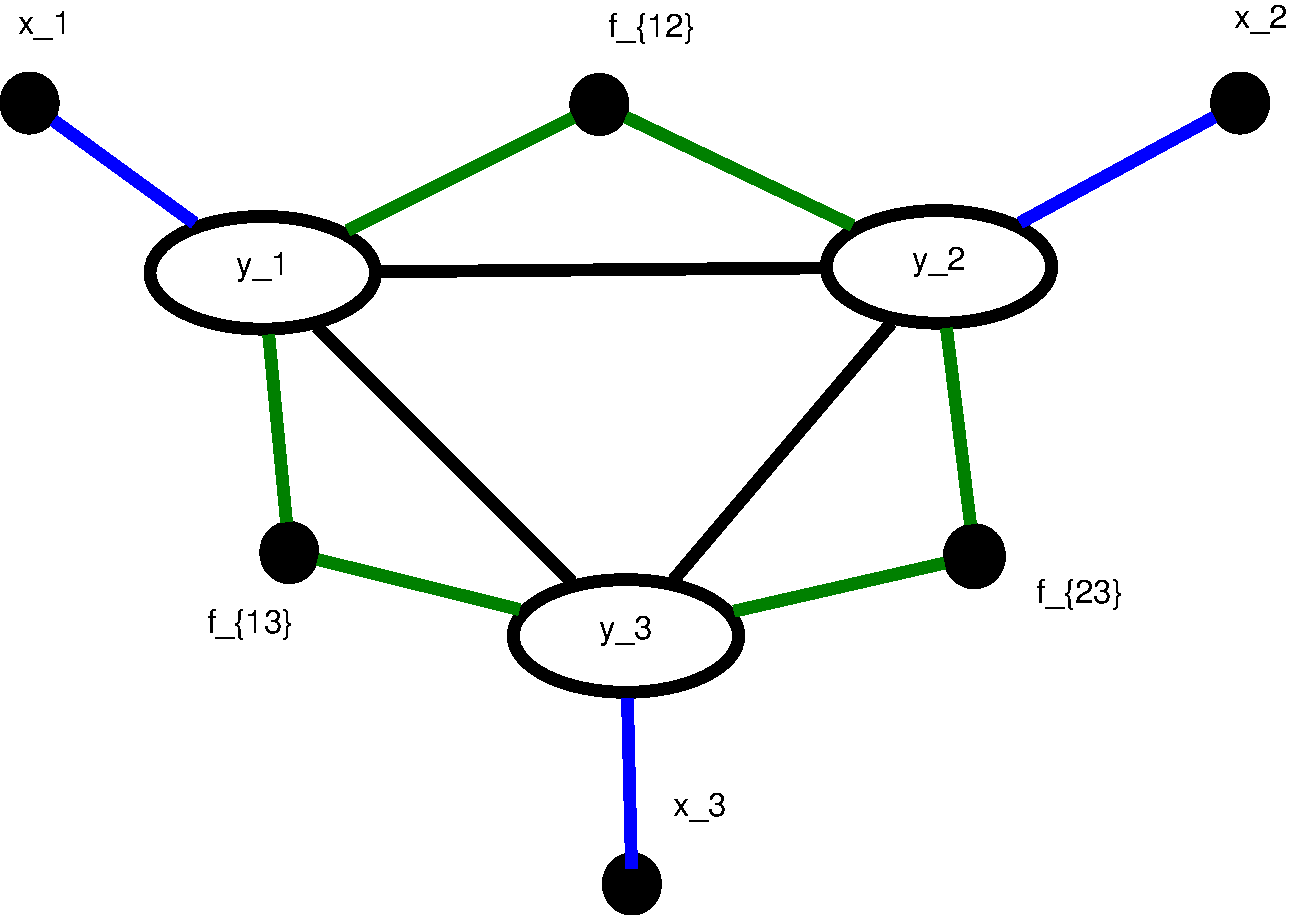
\includegraphics[width=0.5\textwidth]{fig/CRF-fig.pdf}
	\caption{The CRF model of the crime rate $y_i$ for each grid $g_i$.}
	\label{fig:crf}
\end{figure}



In the CRF model, we factorize the probability distribution of $y$ to a series of potential functions $\psi$ on the clique. 
\begin{equation}
	P(Y) = \frac{1}{Z} \prod_{ c \in C} \psi(c)
\end{equation}

Use $C_1$ to denote the set of cliques of size 1 with the form $\langle y_i \rangle$, and $C_2$ to denote size-2 clique. We define the potential function as follows:

\begin{align}
	\psi_{C_1} = &exp( - |y_i - \demow^T \cdot \x_i| )  \forall i \in [1, n], {g_i} \in C_1, \\
	\psi_{C_2} = & exp( - |y_i - y_j - \w^T \cdot \f_{i,j}| )  \forall i,j \in [1, n], {g_i, g_j} \in C_2, 
\end{align}
where $\demow$ and $\w$ are all positive coefficients.

The distribution of $Y$ is given by 
\begin{equation}
	P(Y) =  \frac{1}{Z} \left[ \prod_{i=1}^n \psi_{C_1}(y_i) \times \prod_{i=1}^n \prod_{j=i}^n \psi_{C_2}(y_i, y_j) \right]
\end{equation}
\begin{equation}
	P(Y) =  \frac{1}{Z} exp  \left( - \sum_{i=1}^n |y_i - \demow^T \cdot \x_i|  - \sum_{i=1}^n\sum_{j=i}^n |y_i - y_j - \w^T \cdot \f_{i,j}| \right)
	\label{eq:PY}
\end{equation}


The inference of $CRF$ model is given in the Appendix~\ref{apdx:crf}, and we refer interested reader there.




\section{Graphcial Model Solve Other Proposed Problems}



The graphical model is not only useful to solve inference problem on nodes using links, but also able to solve other problems.



\subsection{Understand links using nodes.}

In a graphical model shown in Figure~\ref{fig:crf}, we can estimate the flow $f_{ij}$ using the nodal attributes $y_i$ and $\x_i$ as well.


This problem answers important questions about the link. For example, we can answer when two regions are becoming very dissimilar in $\x$, what will happend to the taxi interaction between them? What about the LEHD flow.



\subsection{Understand the causal structures}


Graphical model also helps us understand the real dependency structure of node property and flow between nodes.
The assumptions that crime is neighboring community will influence crime in focal community is  over-simplified. Actually, we do not know what impacts crime in focal community. It is very likely to be nodal properties in neighboring communites that impacts crime in focal community. There are various explanations behind, as shown in Figure~\ref{fig:crf-assump}.



\begin{figure}[h]
\centering
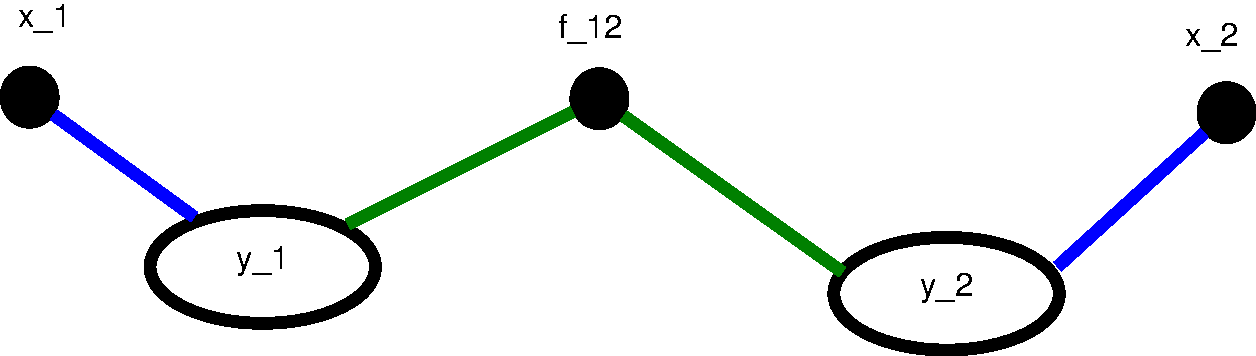
\includegraphics[width=0.45\textwidth]{fig/CRF-base.pdf}
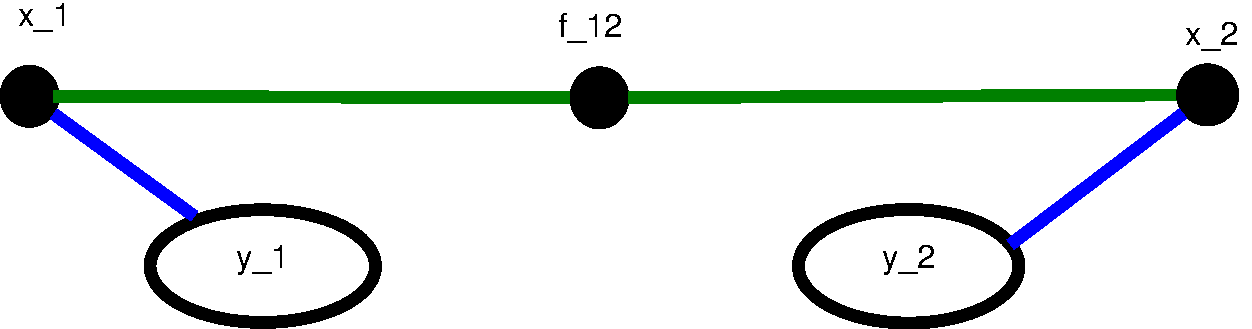
\includegraphics[width=0.45\textwidth]{fig/CRF-impr.pdf}
\caption{Various assumptions on interations behind the inference problem.}
\label{fig:crf-assump}
\end{figure}


